\documentclass[twoside]{book}

% Packages required by doxygen
\usepackage{fixltx2e}
\usepackage{calc}
\usepackage{doxygen}
\usepackage[export]{adjustbox} % also loads graphicx
\usepackage{graphicx}
\usepackage[utf8]{inputenc}
\usepackage{makeidx}
\usepackage{multicol}
\usepackage{multirow}
\PassOptionsToPackage{warn}{textcomp}
\usepackage{textcomp}
\usepackage[nointegrals]{wasysym}
\usepackage[table]{xcolor}

% Font selection
\usepackage[T1]{fontenc}
\usepackage[scaled=.90]{helvet}
\usepackage{courier}
\usepackage{amssymb}
\usepackage{sectsty}
\renewcommand{\familydefault}{\sfdefault}
\allsectionsfont{%
  \fontseries{bc}\selectfont%
  \color{darkgray}%
}
\renewcommand{\DoxyLabelFont}{%
  \fontseries{bc}\selectfont%
  \color{darkgray}%
}
\newcommand{\+}{\discretionary{\mbox{\scriptsize$\hookleftarrow$}}{}{}}

% Page & text layout
\usepackage{geometry}
\geometry{%
  a4paper,%
  top=2.5cm,%
  bottom=2.5cm,%
  left=2.5cm,%
  right=2.5cm%
}
\tolerance=750
\hfuzz=15pt
\hbadness=750
\setlength{\emergencystretch}{15pt}
\setlength{\parindent}{0cm}
\setlength{\parskip}{3ex plus 2ex minus 2ex}
\makeatletter
\renewcommand{\paragraph}{%
  \@startsection{paragraph}{4}{0ex}{-1.0ex}{1.0ex}{%
    \normalfont\normalsize\bfseries\SS@parafont%
  }%
}
\renewcommand{\subparagraph}{%
  \@startsection{subparagraph}{5}{0ex}{-1.0ex}{1.0ex}{%
    \normalfont\normalsize\bfseries\SS@subparafont%
  }%
}
\makeatother

% Headers & footers
\usepackage{fancyhdr}
\pagestyle{fancyplain}
\fancyhead[LE]{\fancyplain{}{\bfseries\thepage}}
\fancyhead[CE]{\fancyplain{}{}}
\fancyhead[RE]{\fancyplain{}{\bfseries\leftmark}}
\fancyhead[LO]{\fancyplain{}{\bfseries\rightmark}}
\fancyhead[CO]{\fancyplain{}{}}
\fancyhead[RO]{\fancyplain{}{\bfseries\thepage}}
\fancyfoot[LE]{\fancyplain{}{}}
\fancyfoot[CE]{\fancyplain{}{}}
\fancyfoot[RE]{\fancyplain{}{\bfseries\scriptsize Generated by Doxygen }}
\fancyfoot[LO]{\fancyplain{}{\bfseries\scriptsize Generated by Doxygen }}
\fancyfoot[CO]{\fancyplain{}{}}
\fancyfoot[RO]{\fancyplain{}{}}
\renewcommand{\footrulewidth}{0.4pt}
\renewcommand{\chaptermark}[1]{%
  \markboth{#1}{}%
}
\renewcommand{\sectionmark}[1]{%
  \markright{\thesection\ #1}%
}

% Indices & bibliography
\usepackage{natbib}
\usepackage[titles]{tocloft}
\setcounter{tocdepth}{3}
\setcounter{secnumdepth}{5}
\makeindex

% Hyperlinks (required, but should be loaded last)
\usepackage{ifpdf}
\ifpdf
  \usepackage[pdftex,pagebackref=true]{hyperref}
\else
  \usepackage[ps2pdf,pagebackref=true]{hyperref}
\fi
\hypersetup{%
  colorlinks=true,%
  linkcolor=blue,%
  citecolor=blue,%
  unicode%
}

% Custom commands
\newcommand{\clearemptydoublepage}{%
  \newpage{\pagestyle{empty}\cleardoublepage}%
}

\usepackage{caption}
\captionsetup{labelsep=space,justification=centering,font={bf},singlelinecheck=off,skip=4pt,position=top}

%===== C O N T E N T S =====

\begin{document}

% Titlepage & ToC
\hypersetup{pageanchor=false,
             bookmarksnumbered=true,
             pdfencoding=unicode
            }
\pagenumbering{alph}
\begin{titlepage}
\vspace*{7cm}
\begin{center}%
{\Large Digital Image Library }\\
\vspace*{1cm}
{\large Generated by Doxygen 1.8.13}\\
\end{center}
\end{titlepage}
\clearemptydoublepage
\pagenumbering{roman}
\tableofcontents
\clearemptydoublepage
\pagenumbering{arabic}
\hypersetup{pageanchor=true}

%--- Begin generated contents ---
\chapter{Class Index}
\section{Class List}
Here are the classes, structs, unions and interfaces with brief descriptions\+:\begin{DoxyCompactList}
\item\contentsline{section}{\hyperlink{classImageBuffer}{Image\+Buffer} \\*Image Buffer used for holding individual Pixel information }{\pageref{classImageBuffer}}{}
\item\contentsline{section}{\hyperlink{structPixel1}{Pixel1} }{\pageref{structPixel1}}{}
\item\contentsline{section}{\hyperlink{structPixel24}{Pixel24} }{\pageref{structPixel24}}{}
\item\contentsline{section}{\hyperlink{structPixel48}{Pixel48} }{\pageref{structPixel48}}{}
\item\contentsline{section}{\hyperlink{structPixelBuffer}{Pixel\+Buffer} }{\pageref{structPixelBuffer}}{}
\end{DoxyCompactList}

\chapter{File Index}
\section{File List}
Here is a list of all files with brief descriptions\+:\begin{DoxyCompactList}
\item\contentsline{section}{\hyperlink{ImageBuffer_8c}{Image\+Buffer.\+c} }{\pageref{ImageBuffer_8c}}{}
\item\contentsline{section}{\hyperlink{ImageBuffer_8h}{Image\+Buffer.\+h} }{\pageref{ImageBuffer_8h}}{}
\item\contentsline{section}{\hyperlink{ImageBufferMacros_8h}{Image\+Buffer\+Macros.\+h} }{\pageref{ImageBufferMacros_8h}}{}
\item\contentsline{section}{\hyperlink{main_8c}{main.\+c} }{\pageref{main_8c}}{}
\item\contentsline{section}{\hyperlink{Pixel_8c}{Pixel.\+c} }{\pageref{Pixel_8c}}{}
\item\contentsline{section}{\hyperlink{Pixel_8h}{Pixel.\+h} \\*Define Pixel Object }{\pageref{Pixel_8h}}{}
\end{DoxyCompactList}

\chapter{Class Documentation}
\hypertarget{structImageBuffer}{}\section{Image\+Buffer Class Reference}
\label{structImageBuffer}\index{Image\+Buffer@{Image\+Buffer}}


Image Buffer used for holding individual Pixel information.  




{\ttfamily \#include $<$Image\+Buffer.\+h$>$}

\subsection*{Public Attributes}
\begin{DoxyCompactItemize}
\item 
\mbox{\Hypertarget{structImageBuffer_acfaa0fdac0150fc07cbcbcc857e8c18f}\label{structImageBuffer_acfaa0fdac0150fc07cbcbcc857e8c18f}} 
Pixel $\ast$ \hyperlink{structImageBuffer_acfaa0fdac0150fc07cbcbcc857e8c18f}{buffer}
\begin{DoxyCompactList}\small\item\em Buffer to store pixel data. \end{DoxyCompactList}\end{DoxyCompactItemize}


\subsection{Detailed Description}
Image Buffer used for holding individual Pixel information. 

Buffer that stores pixel data to be used for holding pixel data that is used to write, read, and manipulate Pixel data from images. 

The documentation for this class was generated from the following file\+:\begin{DoxyCompactItemize}
\item 
include/\hyperlink{ImageBuffer_8h}{Image\+Buffer.\+h}\end{DoxyCompactItemize}

\chapter{File Documentation}
\hypertarget{ImageBuffer_8h}{}\section{include/\+Image\+Buffer.h File Reference}
\label{ImageBuffer_8h}\index{include/\+Image\+Buffer.\+h@{include/\+Image\+Buffer.\+h}}
{\ttfamily \#include $<$limits.\+h$>$}\newline
{\ttfamily \#include \char`\"{}Pixel.\+h\char`\"{}}\newline
Include dependency graph for Image\+Buffer.\+h\+:\nopagebreak
\begin{figure}[H]
\begin{center}
\leavevmode
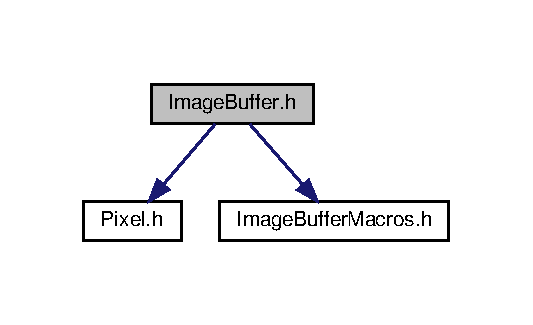
\includegraphics[width=195pt]{ImageBuffer_8h__incl}
\end{center}
\end{figure}
\subsection*{Classes}
\begin{DoxyCompactItemize}
\item 
class \hyperlink{structImageBuffer}{Image\+Buffer}
\begin{DoxyCompactList}\small\item\em Image Buffer used for holding individual Pixel information. \end{DoxyCompactList}\end{DoxyCompactItemize}
\subsection*{Typedefs}
\begin{DoxyCompactItemize}
\item 
\mbox{\Hypertarget{ImageBuffer_8h_a2171a13893e19f5135f55b19f68e44c3}\label{ImageBuffer_8h_a2171a13893e19f5135f55b19f68e44c3}} 
typedef struct \hyperlink{structImageBuffer}{Image\+Buffer} {\bfseries Image\+Buffer}
\end{DoxyCompactItemize}
\subsection*{Functions}
\begin{DoxyCompactItemize}
\item 
void \hyperlink{ImageBuffer_8h_ab3ee621c568dd70d45e0d7522be1d195}{init\+Heap\+Buffer} (\hyperlink{structImageBuffer}{Image\+Buffer} $\ast$object, int width, int height)
\begin{DoxyCompactList}\small\item\em Initialize the $\ast$heap\+Buffer. \end{DoxyCompactList}\end{DoxyCompactItemize}


\subsection{Function Documentation}
\mbox{\Hypertarget{ImageBuffer_8h_ab3ee621c568dd70d45e0d7522be1d195}\label{ImageBuffer_8h_ab3ee621c568dd70d45e0d7522be1d195}} 
\index{Image\+Buffer.\+h@{Image\+Buffer.\+h}!init\+Heap\+Buffer@{init\+Heap\+Buffer}}
\index{init\+Heap\+Buffer@{init\+Heap\+Buffer}!Image\+Buffer.\+h@{Image\+Buffer.\+h}}
\subsubsection{\texorpdfstring{init\+Heap\+Buffer()}{initHeapBuffer()}}
{\footnotesize\ttfamily void init\+Heap\+Buffer (\begin{DoxyParamCaption}\item[{\hyperlink{structImageBuffer}{Image\+Buffer} $\ast$}]{object,  }\item[{int}]{width,  }\item[{int}]{height }\end{DoxyParamCaption})}



Initialize the $\ast$heap\+Buffer. 


\begin{DoxyParams}{Parameters}
{\em object} & The \hyperlink{structImageBuffer}{Image\+Buffer} Struct \\
\hline
{\em width} & Image Width \\
\hline
{\em height} & Image Height \\
\hline
\end{DoxyParams}

\hypertarget{Pixel_8h}{}\section{include/\+Pixel.h File Reference}
\label{Pixel_8h}\index{include/\+Pixel.\+h@{include/\+Pixel.\+h}}


Define Pixel Object.  


{\ttfamily \#include $<$stdint.\+h$>$}\newline
Include dependency graph for Pixel.\+h\+:\nopagebreak
\begin{figure}[H]
\begin{center}
\leavevmode
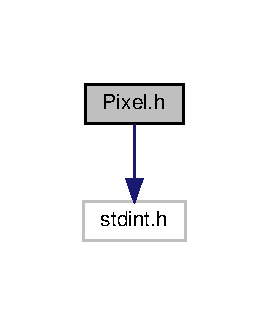
\includegraphics[width=160pt]{Pixel_8h__incl}
\end{center}
\end{figure}
This graph shows which files directly or indirectly include this file\+:
\nopagebreak
\begin{figure}[H]
\begin{center}
\leavevmode
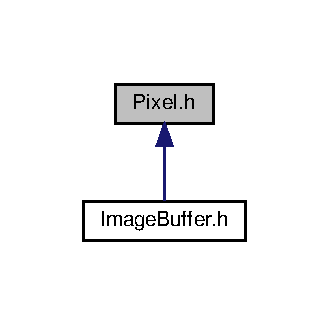
\includegraphics[width=187pt]{Pixel_8h__dep__incl}
\end{center}
\end{figure}
\subsection*{Classes}
\begin{DoxyCompactItemize}
\item 
struct \hyperlink{structPixel1}{Pixel1}
\item 
struct \hyperlink{structPixel24}{Pixel24}
\item 
struct \hyperlink{structPixel48}{Pixel48}
\end{DoxyCompactItemize}
\subsection*{Macros}
\begin{DoxyCompactItemize}
\item 
\mbox{\Hypertarget{Pixel_8h_a1c7242e36bf21082fbfb88f179f3e2e0}\label{Pixel_8h_a1c7242e36bf21082fbfb88f179f3e2e0}} 
\#define \hyperlink{Pixel_8h_a1c7242e36bf21082fbfb88f179f3e2e0}{Pixel8}~uint32\+\_\+t
\begin{DoxyCompactList}\small\item\em Pixel8 is a uint32\+\_\+t capable of representing 8-\/bit grayscale and 8-\/bit color. \end{DoxyCompactList}\item 
\mbox{\Hypertarget{Pixel_8h_a203ea1ec977221ccab14a5f6004e1c07}\label{Pixel_8h_a203ea1ec977221ccab14a5f6004e1c07}} 
\#define \hyperlink{Pixel_8h_a203ea1ec977221ccab14a5f6004e1c07}{Pixel16}~uint64\+\_\+t
\begin{DoxyCompactList}\small\item\em Pixel16 is an uint64\+\_\+t capable of representing 16-\/bit color depth (High color). \end{DoxyCompactList}\item 
\mbox{\Hypertarget{Pixel_8h_af981fca931a8e62348ea5f2d0121e8d4}\label{Pixel_8h_af981fca931a8e62348ea5f2d0121e8d4}} 
\#define {\bfseries R\+G\+B\+A2\+Pixel8}(red,  green,  blue,  alpha)~((((((red) $<$$<$ 24)) $\vert$ ((green) $<$$<$ 16)) $\vert$ ((blue) $<$$<$ 8)) $\vert$ ((alpha) $<$$<$ 0))
\item 
\#define \hyperlink{Pixel_8h_a7a004c69cfd71bf4847f7e00f8d4d92a}{R\+G\+B2\+Pixel}(red,  green,  blue)~R\+G\+B\+A2\+Pixel(red, green, blue, 0)
\begin{DoxyCompactList}\small\item\em A macro that returns and integer from R\+GB values. \end{DoxyCompactList}\item 
\#define \hyperlink{Pixel_8h_a80818d1694127e573190aa454075ecf4}{get\+Red\+Component}(pixel)~((pixel) \& (0x\+F\+F000000)) $>$$>$ 24
\begin{DoxyCompactList}\small\item\em A macro that returns the red color component from the pixel. \end{DoxyCompactList}\item 
\#define \hyperlink{Pixel_8h_a24c65d670b2a4d983b5274652a43ce9f}{get\+Green\+Component}(pixel)~((pixel) \& (0x\+F\+F0000)) $>$$>$ 16
\begin{DoxyCompactList}\small\item\em A macro that returns the green color component from the pixel. \end{DoxyCompactList}\item 
\#define \hyperlink{Pixel_8h_ab660afc642f68a0f25f8e8e84ee26044}{get\+Blue\+Component}(pixel)~((pixel) \& (0x\+F\+F00)) $>$$>$ 8
\begin{DoxyCompactList}\small\item\em A macro that returns the blue color component from the pixel. \end{DoxyCompactList}\item 
\#define \hyperlink{Pixel_8h_ad1b78c0c4353eba81bd1a627f595964d}{get\+Alpha\+Component}(pixel)~((pixel) \& (0x\+F\+F)) $>$$>$ 0
\begin{DoxyCompactList}\small\item\em A macro that returns the blue color component from the pixel. \end{DoxyCompactList}\end{DoxyCompactItemize}
\subsection*{Typedefs}
\begin{DoxyCompactItemize}
\item 
\mbox{\Hypertarget{Pixel_8h_a9dd7a610290467ff3a144037e8dc8eda}\label{Pixel_8h_a9dd7a610290467ff3a144037e8dc8eda}} 
typedef struct \hyperlink{structPixel1}{Pixel1} {\bfseries Pixel1}
\item 
\mbox{\Hypertarget{Pixel_8h_a9bda2e15792ae05629fd3571f20cde95}\label{Pixel_8h_a9bda2e15792ae05629fd3571f20cde95}} 
typedef struct \hyperlink{structPixel24}{Pixel24} {\bfseries Pixel24}
\item 
\mbox{\Hypertarget{Pixel_8h_a7988b82506d0cd1b507c770e6b566171}\label{Pixel_8h_a7988b82506d0cd1b507c770e6b566171}} 
typedef struct \hyperlink{structPixel48}{Pixel48} {\bfseries Pixel48}
\end{DoxyCompactItemize}


\subsection{Detailed Description}
Define Pixel Object. 

Pixel is an unsigned int that stores individual values as a single value This also contains macros for manipulating elementary data types and treating them as Pixel data types. 

\subsection{Macro Definition Documentation}
\mbox{\Hypertarget{Pixel_8h_ad1b78c0c4353eba81bd1a627f595964d}\label{Pixel_8h_ad1b78c0c4353eba81bd1a627f595964d}} 
\index{Pixel.\+h@{Pixel.\+h}!get\+Alpha\+Component@{get\+Alpha\+Component}}
\index{get\+Alpha\+Component@{get\+Alpha\+Component}!Pixel.\+h@{Pixel.\+h}}
\subsubsection{\texorpdfstring{get\+Alpha\+Component}{getAlphaComponent}}
{\footnotesize\ttfamily \#define get\+Alpha\+Component(\begin{DoxyParamCaption}\item[{}]{pixel }\end{DoxyParamCaption})~((pixel) \& (0x\+F\+F)) $>$$>$ 0}



A macro that returns the blue color component from the pixel. 


\begin{DoxyParams}{Parameters}
{\em pixel} & is the pixel color value \\
\hline
\end{DoxyParams}
\begin{DoxyReturn}{Returns}
unsigned char that represents a the blue component of the pixel 
\end{DoxyReturn}
\mbox{\Hypertarget{Pixel_8h_ab660afc642f68a0f25f8e8e84ee26044}\label{Pixel_8h_ab660afc642f68a0f25f8e8e84ee26044}} 
\index{Pixel.\+h@{Pixel.\+h}!get\+Blue\+Component@{get\+Blue\+Component}}
\index{get\+Blue\+Component@{get\+Blue\+Component}!Pixel.\+h@{Pixel.\+h}}
\subsubsection{\texorpdfstring{get\+Blue\+Component}{getBlueComponent}}
{\footnotesize\ttfamily \#define get\+Blue\+Component(\begin{DoxyParamCaption}\item[{}]{pixel }\end{DoxyParamCaption})~((pixel) \& (0x\+F\+F00)) $>$$>$ 8}



A macro that returns the blue color component from the pixel. 


\begin{DoxyParams}{Parameters}
{\em pixel} & is the pixel color value \\
\hline
\end{DoxyParams}
\begin{DoxyReturn}{Returns}
unsigned char that represents a the blue component of the pixel 
\end{DoxyReturn}
\mbox{\Hypertarget{Pixel_8h_a24c65d670b2a4d983b5274652a43ce9f}\label{Pixel_8h_a24c65d670b2a4d983b5274652a43ce9f}} 
\index{Pixel.\+h@{Pixel.\+h}!get\+Green\+Component@{get\+Green\+Component}}
\index{get\+Green\+Component@{get\+Green\+Component}!Pixel.\+h@{Pixel.\+h}}
\subsubsection{\texorpdfstring{get\+Green\+Component}{getGreenComponent}}
{\footnotesize\ttfamily \#define get\+Green\+Component(\begin{DoxyParamCaption}\item[{}]{pixel }\end{DoxyParamCaption})~((pixel) \& (0x\+F\+F0000)) $>$$>$ 16}



A macro that returns the green color component from the pixel. 


\begin{DoxyParams}{Parameters}
{\em pixel} & is the pixel color value \\
\hline
\end{DoxyParams}
\begin{DoxyReturn}{Returns}
unsigned char that represents a the green component of the pixel 
\end{DoxyReturn}
\mbox{\Hypertarget{Pixel_8h_a80818d1694127e573190aa454075ecf4}\label{Pixel_8h_a80818d1694127e573190aa454075ecf4}} 
\index{Pixel.\+h@{Pixel.\+h}!get\+Red\+Component@{get\+Red\+Component}}
\index{get\+Red\+Component@{get\+Red\+Component}!Pixel.\+h@{Pixel.\+h}}
\subsubsection{\texorpdfstring{get\+Red\+Component}{getRedComponent}}
{\footnotesize\ttfamily \#define get\+Red\+Component(\begin{DoxyParamCaption}\item[{}]{pixel }\end{DoxyParamCaption})~((pixel) \& (0x\+F\+F000000)) $>$$>$ 24}



A macro that returns the red color component from the pixel. 


\begin{DoxyParams}{Parameters}
{\em pixel} & is the pixel color value \\
\hline
\end{DoxyParams}
\begin{DoxyReturn}{Returns}
Unsigned char that represents a the red component of the pixel 
\end{DoxyReturn}
\mbox{\Hypertarget{Pixel_8h_a7a004c69cfd71bf4847f7e00f8d4d92a}\label{Pixel_8h_a7a004c69cfd71bf4847f7e00f8d4d92a}} 
\index{Pixel.\+h@{Pixel.\+h}!R\+G\+B2\+Pixel@{R\+G\+B2\+Pixel}}
\index{R\+G\+B2\+Pixel@{R\+G\+B2\+Pixel}!Pixel.\+h@{Pixel.\+h}}
\subsubsection{\texorpdfstring{R\+G\+B2\+Pixel}{RGB2Pixel}}
{\footnotesize\ttfamily \#define R\+G\+B2\+Pixel(\begin{DoxyParamCaption}\item[{}]{red,  }\item[{}]{green,  }\item[{}]{blue }\end{DoxyParamCaption})~R\+G\+B\+A2\+Pixel(red, green, blue, 0)}



A macro that returns and integer from R\+GB values. 


\begin{DoxyParams}{Parameters}
{\em red} & is the red color value \\
\hline
{\em green} & is the green color value \\
\hline
{\em blue} & is the blue color value \\
\hline
\end{DoxyParams}
\begin{DoxyReturn}{Returns}
integer that represents a specific pixel color without alpha opacity 
\end{DoxyReturn}

%--- End generated contents ---

% Index
\backmatter
\newpage
\phantomsection
\clearemptydoublepage
\addcontentsline{toc}{chapter}{Index}
\printindex

\end{document}
